\documentclass{article}

\usepackage[T2A]{fontenc}
\usepackage[utf8]{inputenc}
\usepackage[russian]{babel}
\usepackage{amsmath}
\usepackage{amssymb}
\usepackage{amsthm}
\usepackage{mathrsfs}
\usepackage{booktabs}
\usepackage{makecell}
\usepackage{multirow}
\usepackage{makecell}
\usepackage{multicol}
\usepackage{placeins}

\usepackage{dan2e}

% Эти четыре строчки, чтобы исправить проблему с компиляцией 
% т.к. не определялся if@Russian, возможно из-за более новой версии babel
\makeatletter
\@ifundefined{@Russian}{\newif\if@Russian \@Russiantrue}{}
\@ifundefined{@TVP}     {\newif\if@TVP    \@TVPfalse}{}
\makeatother

\theoremstyle{definition}
\newtheorem{defi}{Определение}
\theoremstyle{plain}
\newtheorem{remark}{Пример}
\newtheorem{theorem}{Теорема}
\newtheorem{OldTheorem}{Теорема}
\renewcommand{\theOldTheorem}{\Alph{OldTheorem}}

\newtheorem{Theorem}{Теорема}
\renewcommand{\theTheorem}{\arabic{theorem}$^\prime$}

\begin{document}
\raggedbottom
\Volume{505}
\Year{2025}
\Pages{46--49}

\udk{517.54}

\title{Оценка общих и специальных знаний в больших языковых моделях для русского языка посредством воспроизведения энциклопедических статей}

\author{Д.\,А.~Григорьев\Addressmark[1]\Emailmark[1], Д.\,И.~Чернышев\Addressmark[1]\Emailmark[2]}

\Addresstext[1]{Московский государственный университет им.~М.\,В.~Ломоносова, Москва, Россия}

\Emailtext[1]{dagrig14@yandex.ru}

\Emailtext[2]{chdanorbis@yandex.ru}

\markboth{Д.\,А.~Григорьев, Д.\,И.~Чернышев}{Оценка общих и специальных знаний в больших языковых моделях}

\presentedby{Представлено кем-то}

\dateA{16.08.2025}
\dateB{20.08.2025}
\dateC{31.08.2025}

\alttitle{Evaluating general and special knowledge in large language models for Russian language through replication of encyclopedia articles}

\altauthor{D.\,A.~Grigoriev\Addressmark[a]\Emailmark[1], D.\,I.~Chernyshev\Addressmark[a]\Emailmark[2]}

\altAddresstext[a]{Lomonosov Moscow State University, Moscow Center for Fundamental and Applied Mathematics, \\ Moscow, Russian Federation}

\altpresentedby{Presented by Academician of the RAS B.\,S.~Kashin}

\maketitle

\doi{10.31857/S2686954322040117}

\begin{abstract}
В данной работе предложен и реализован бенчмарк WikiBench для оценки аналитических способностей больших языковых моделей при составлении научно-энциклопедических текстов на русском языке. 
\end{abstract}

\begin{keywords}
бенчмарк, Википедия, Рувики, large language model
\end{keywords}

\begin{altabstract}
In this work we propose and implement WikiBench for evaluating the analytical capabilities of large language models in generating scientific and encyclopedic texts in Russian.
\end{altabstract}

\begin{altkeywords}
benchmark, Wikipedia, Ruwiki, large language model
\end{altkeywords}

% ВВЕДЕНИЕ --------
\section*{Введение}

Современные большие языковые модели демонстрируют впечатляющие результаты в генерации текстов различной стилистики и тематики. 
Однако их способности к работе с научными и энциклопедическими материалами остаются малоизученными, особенно для русскоязычных текстов. 
Традиционные методы создания научных статей требуют значительных временных затрат на поиск и анализ информации. 
Если большая языковая модель сможет самостоятельно проводить такие "глубокие" исследования по темам, не входящим в ее первоначальные тренировочные данные, это позволит отказаться от постоянного дообучения моделей
и предложить более эффективный и масштабируемый подход к работе с постоянно обновляющимся научными знаниями.
Существующие методы оценки способностей моделей преимущественно фокусируются на стандартных лингвистических задачах, не уделяя достаточного внимания аналитическим способностям при работе с научными текстами.
Для русского языка эта проблема особенно актуальна из-за ограниченной доступности специализированных оценочных инструментов.

Существует множество бенчмарков на русском языке, охватывающих различные лингвистические задачи для русского языка.
RussianSuperGlue \cite{rsglue} оценивает общее языковое понимание и базовые задачи по обработки естественного языка. 
MERA \cite{mera} обеспечивает единые условия тестирования моделей за счет составления инструкций к генерации для каждой задачи, однако сами задачи ориентированы на проверку общего понимания. 
LIBRA \cite{libra} фокусируется на проверке способности модели к удержанию и извлечению информации из большого контекста, но сосредоточен на коротких ответах, не требующих глубоких рассуждений. 
Ru Arena General \cite{arena} фокусируется на парном сравнении моделей, но фокусируется на общем качестве ответа.
Ping-Pong \cite{pp} оценивает диалоговые способности моделей, что важно для интерактивных систем, но не подходит для оценки способности проводить исследования и писать связные научно-энциклопедические тексты.
При этом остается неохваченным целый класс задач, связанных с глубоким анализом текстов: создание развернутых, структурированных и фактологически точных текстов, подкрепленных большим количеством источников. 

Существующие бенчмарки в ограниченной степени затрагивают критически важные для генерации научно-энциклопедических текстов аспекты, 
такие как умение обобщать информацию из набора документов, планировать структуру будущего текста, соблюдать связанность и логическую последовательность изложения, а также обеспечивать точность и достоверность фактов. 
Одним из ближайших исследований в этой области является ResearchArena \cite{resar}, в которой формализуют построение академического обзора с помощью трех этапов:
обнаружение релевантной литературы, отбор по значимости и организация знаний. Однако этот бенчмарк больше нацелен на проверку способности моделей отбирать и организовывать релевантную информацию
и не затрагивает способности модели генерировать связные научно-энциклопедические тексты.
Также развиваются в направлении похожих задач такие методы как Storm \cite{storm} - он подготавливает статью через создание множества перспектив и диалогов между ними.
Однако это не позволяет в полной мере отследить каждый этап генерации, и дает меньший контроль над параметрами генерации.
Недавнее развитие новых способностей агентов, например появление функции «Deep Research» у OpenAI \cite{deepr}, 
свидетельствует о возрастающем интересе к проведению научных исследования с помощью больших языковых моделей, 
что говорит о необходимости в создании новых подходов к объективной оценке аналитических способностей моделей. 

В данной работе предлагается подход, направленный на создание 
инструментов, позволяющих тестировать, насколько большие языковые модели умеют работать с научно-энциклопедическими текстами.
В рамках исследования:
\begin{enumerate}

    \item Был реализован автоматический метод обработки html-кода статей в стиле Википедии и собран размеченный набор данных на основе интернет-энциклопедии «Рувики»
    
    \item Был разработан и протестирован открытый бенчмарк WikiBench, позволяющий измерять качество модели на задачах, требующих глубокого анализа текста.

\end{enumerate}

% СБОР ДАННЫХ --------
\section*{Сбор данных}

Для построения бенчмарка, направленного на оценку способности языковых моделей к работе с источниками к статьям, необходимо подготовить корпус текстов, который будет использоваться в генерации. 
В качестве источника были выбраны статьи интернет энциклопедии <<Рувики>> - российский аналог Википедии. Выбор сделан в пользу стилистики Википедии по той причине, что этот жанр
одновременно требует фактологической точности, полноты анализа и понимания контекста, что хорошо соотносится с направлением исследования этой работы.

Переход на Рувики обоснован тем, что российская википедия содержит больше ссылок на русскоязычные источники, а также проводит более строгую фильтрацию текстов, 
что позволяет положиться на нее, как на более надежный эталон для оценки качества генерации статей.

Процесс получения данных включал следующие шаги:

\begin{enumerate}

    \item \textbf{Выбор статей}: вручную были отобраны статьи на разнообразные темы, 
    содержащие достаточное количество ссылок на внешние источники.
    
    \item \textbf{Загрузка источников}: для каждой статьи были автоматически собраны доступные источники, на которые она ссылается. 
    Загрузка производилась с помощью Python-модуля \texttt{newspaper3k}.
    
    \item \textbf{Разбиение на сниппеты}: для удобства работы с текстами, а также в связи с ограничениями контекстного окна большинства языковых моделей, 
    все тексты были разбиты на небольшие фрагменты длиной $\approx 600$ слов. 
    При необходимости в процессе тестирования модели можно расширить окно контекста, подключив соседние сниппеты того же источника.

\end{enumerate}

\begin{figure}[ht!]
  \centering
  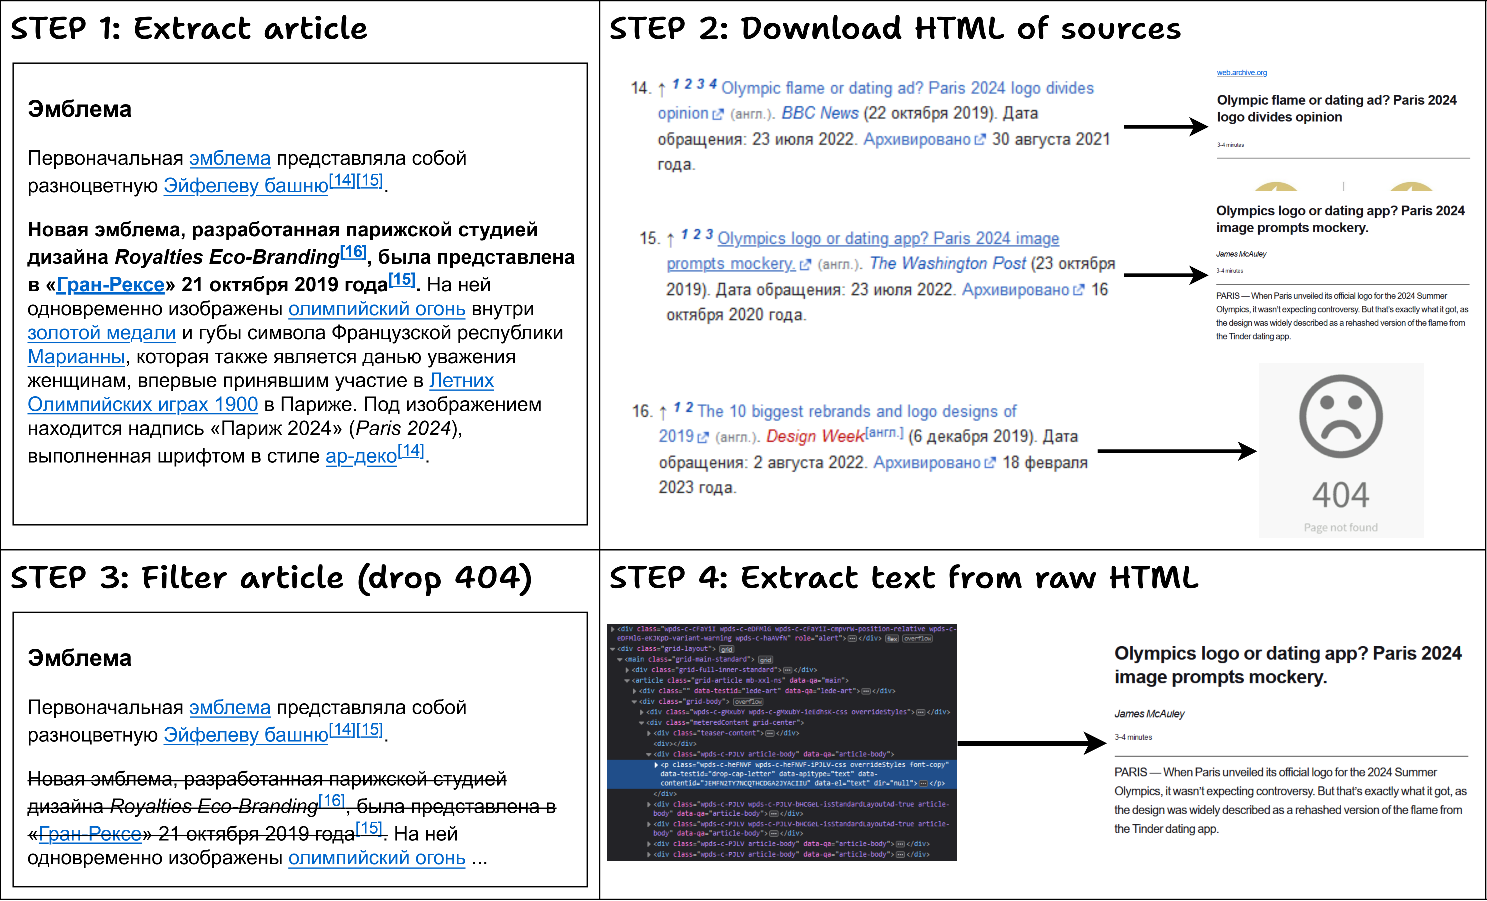
\includegraphics[width=0.6\textwidth]{figures/Source_extract.png}%
  \caption{Извлечение источников}
  \label{fig:source}
\end{figure}

\begin{figure}[ht!]
  \centering
  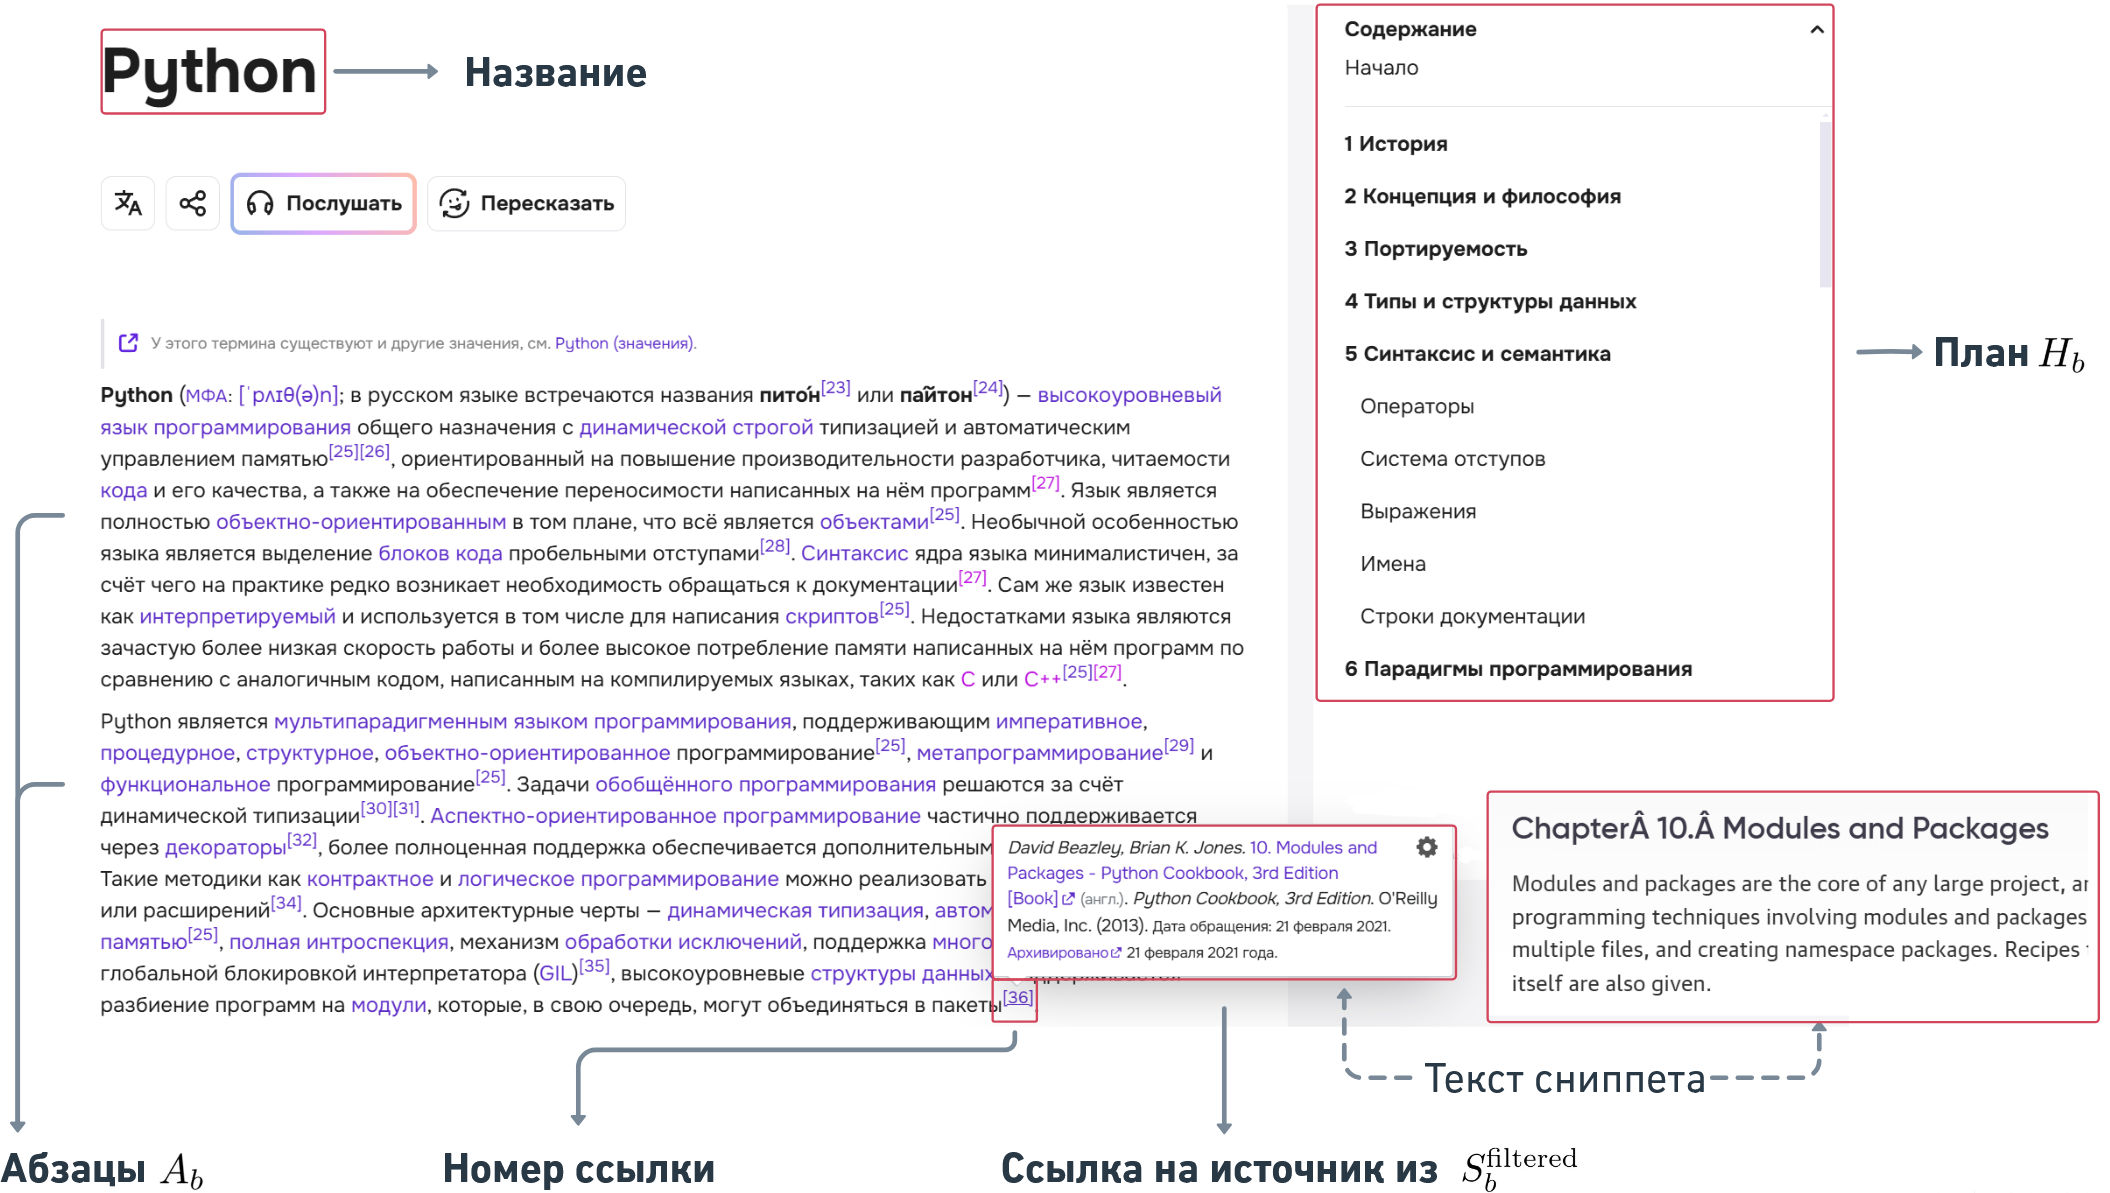
\includegraphics[width=0.6\textwidth]{figures/article_entities.png}%
  \caption{Основные сущности статьи}
  \label{fig:article}
\end{figure}

На этапе получения данных осуществляется первичное извлечение информации из выбранной статьи и сбор связанных с ней источников. На рисунке \ref{fig:source} показана краткая схема извлечения текстов источников.
В качестве исходного корпуса берётся подмножество статей Википедии \(B\).
Формально для каждой статьи \(b\in B\) задаётся её тема \(\theta_b\) и набор заголовков \(H_b=\{(h_i,l_i)\}\) с уровнями вложенности, а также набор абзацев \(A_b\) по секциям.
Извлечение HTML-кода статьи выполняется с помощью стандартных инструментов Python-модулей\footnote{https://beautiful-soup-4.readthedocs.io/en/latest/},\footnote{https://requests.readthedocs.io/en/latest/index.html}. 
Полученный текст структурируется путем разбиения на фрагменты, соответствующие вложенным заголовкам (H1, H2, H3 и т.д.), что позволяет сохранить как содержательную часть статьи, так и её иерархическую организацию. 
Далее из раздела «Примечания» автоматически извлекаются все внешние ссылки, на которые статья делает отсылки. После этого проводится проверка доступности каждой ссылки: в случае обнаружения ошибок 
(например, код 404) такие ссылки исключаются из дальнейшей обработки, а связанный с ними текст удаляется, оставляя только те источники, которые действительно доступны,
то есть источники \(S_b\) к статье фильтруются: из них выбирается подмножество \(S_b^{\mathrm{filtered}}=\{(s_q,t_q)\}\), для которых получен текст \(t_q\). 
Рисунок \ref{fig:article} иллюстрирует схематичное разбиение статьи\footnote{https://ru.ruwiki.ru/wiki/Python} на ключевые сущности, используемые в дальнейшей обработке.
На этапе обработки данных выполняется фильтрация текста для обеспечения его корректной интерпретации моделью. 
Каждая сноска, обозначенная цифрами в квадратных скобках (например, [1], [2]), сопоставляется с конкретной ссылкой, соответствующей одному из доступных источников. 
То есть задано отображение по формуле \eqref{func}:
\begin{equation}\label{func}
  F_b: S_b \to H_b \times A_b
\end{equation}
связывающее каждый источник с конкретным заголовком и абзацем.
Это позволяет точно определить позицию ссылки в тексте статьи и использовать её для последующей фильтрации. 
На основании \(S_b^{\mathrm{filtered}}\) формируются очищенные множества абзацев \(A_b^{\mathrm{filtered}}\) и заголовков \(H_b^{\mathrm{filtered}}\), 
то есть остаётся только тот контент, подкреплённый извлечёнными источниками; всё прочее удаляется. 

Источники фильтруются по наличию извлечённого текста: сохраняются только те \(s_q\) из \(S_b\), для которых удалось получить текст \(t_q\) объёмом не менее 1500 символов - 
это условие отсекает «шумовые» ответы с HTML-страниц вроде ошибок (например, error 404) или слишком короткие фрагменты. 
Абзацы очищаются следующим образом: в \(A_b^{\mathrm{filtered}}\) остаются только те абзацы, в которых присутствует хотя бы одна ссылка на источник из \(S_b^{\mathrm{filtered}}\); 
абзацы без ссылок или со ссылками, для которых текст не был получен, удаляются. 
Аналогично формируется \(H_b^{\mathrm{filtered}}\) - только те заголовки, под которыми остался поддерживаемый источниками текст (хотя бы один абзац).
В результате из статьи удаляются фрагменты, опирающиеся на источники, текст которых не удалось получить, оставляя только те части текста,
которые подкреплены достоверными и доступными источниками. Характеристики собранного корпуса представлены в таблице \ref{tab:dataset}.

\begin{table}[ht!]
  \centering
  \caption{Основные характеристики собранного датасета}
  \label{tab:dataset}
  \begin{tabular}{lcc}
    \hline
    \textbf{Показатель} & \textbf{WikiBench} & \textbf{ResearchArena} \\
    \hline
    Количество статей                             & 100 & 7,952\\
    \hline
    Количество скачанных источников               & 5828 & 12,034,505\\
    \hline
    Общее число сниппетов                         & 13704 & -\\
    \hline
    Средний размер плана (число заголовков)       & 37 & -\\
    \hline
    Средний размер секции (число слов)            & 112 & -\\
    \hline
  \end{tabular}
\end{table}

% МЕТОДИКА ОЦЕНКИ --------
\section*{Методика оценки}

Для объективной оценки способностей языковых моделей генерировать научно-энциклопедические тексты, необходимо воспроизвести реальный процесс подготовки энциклопедического контента:
\begin{enumerate}

    \item \textbf{Отбор релевантных источников}: модель получает заголовок статьи и набор текстовых фрагментов, среди которых необходимо идентифицировать и ранжировать по степени значимости материалы, соответствующие тематике. 
    
    \item \textbf{Построение структуры будущей статьи}: на основании темы и отобранных источников модель формирует план с выделением основных разделов в стиле Википедии.
    
    \item \textbf{Генерация текста}: материалы статьи распределяются по разделам, после чего для каждого раздела порождается обобщение его релевантных материалов

\end{enumerate}
Каждому этапу соответствует специализированный набор метрик, позволяющий количественно измерить качество выполнения конкретной подзадачи. 
Детальное описание методик оценки для каждого из этапов представлено в следующих разделах.
\subsection*{Ранжирование источников.}
Исходя из недавно проведенных исследований \cite{rerank}, предложенный далее подход является одним из наиболее эффективных.
Первоначально для каждой статьи на основе ее названия генерируется ее краткое описание. 
Описание генерируется на русском и английском языках, так как тексты источников тоже представлены в двух языковых вариантах. 
Запросы на обоих языках далее объединяются в единый текстовый запрос к системе поиска, основанной на BM25. 

Проводились эксперименты с двумя вариантами составления запроса:
\begin{enumerate}

    \item \textbf{Заранее сгенерированный запрос по названию и заголовкам второго уровня}: для чистой оценки способности ранжирования проверяется и другой вариант с использованием «сильной» языковой модели llama3-70b: 
    ей передаются в подсказке заголовки второго уровня текущей статьи, и по ним генерируется аннотация.  
    
    \item \textbf{Запрос, сгенерированный по названию посредством оцениваемой модели}: описание генерируется исключительно по названию статьи самой оцениваемой моделью без дополнительных заголовков.
    Таким образом LLM полностью отвечает за качество выдачи и самостоятельно решает, какой поисковый запрос лучше сформулировать для BM25.

\end{enumerate}
Так получается описание, с упомянутыми основными заголовками или основанные только на названии статьи, как показано в таблице \ref{tab:c++} (только на русском языке).

\begin{table}[ht!]
\centering
\begin{tabular}{|p{0.15\linewidth}|p{0.75\linewidth}|}
\hline
\makecell{\textbf{Вариант} \\ \textbf{аннотации}} & \makecell{\textbf{Текст}} \\ \hline

\textbf{Генерация по заголовкам} & Статья "C++" представляет собой обзор языка программирования C++, его истории, структуры и особенностей. 
В ней рассматриваются основные аспекты языка, включая его стандартную библиотеку, отличия от языка C и дальнейшее развитие. 
Кроме того, статья содержит примеры программ на C++, сравнение с альтернативными языками программирования, а также критический анализ и обсуждение влияния C++ на развитие программирования и существующие альтернативы. 
Статья предназначена для читателей, интересующихся языком C++ и его ролью в современном программировании. \\ \hline

\textbf{Генерация по названию}   & Статья "C++" может быть посвящена языку программирования C++, являющимся одним из наиболее популярных и широко используемых языков программирования в мире.
В статье могут быть рассмотрены основы языка, его история, синтаксис и особенности, а также его применение в различных областях, таких как разработка операционных систем, игр и веб-приложений. 
Кроме того, статья может содержать информацию о стандартах и библиотеках C++, а также о его сравнении с другими языками программирования. 
Статья может быть полезна как для начинающих программистов, так и для опытных специалистов, которые хотят углубить свои знания о языке C++.
Статья также может включать примеры кода и практические советы по использованию C++ в реальных проектах.  \\ \hline

\end{tabular}
\caption{Сравнение описаний статьи «C++» в двух вариантах}
\label{tab:c++}
\end{table}

На основе полученного запроса посредством BM25 отбираются наиболее релевантные сниппеты: набор кандидатов-документов. Отобранные документы последовательно передаются большой языковой модели, которая должна определить каждый сниппет как релевантный (ответ «да») или нерелевантный (ответ «нет»). 
Для получения численных оценок сравниваются названия статей, к которым относятся документы из выдачи и название статьи, для которой происходит отбор текстов-источников. 
Берется логарифмическая вероятность токенов в ответе модели: если это был утвердительный ответ, то берется сама вероятность P(«да»), если отрицательный, то берется обратное значение, то есть 1 – P(«нет»).
Если модель взяла правильный документ (он относится к текущей обрабатываемой статье и модель ответила <<да>>), то данный документ получает значение 1 - он релевантный. В противном случае, документу присваивается значение 0. 
Такой подход позволяет ранжировать выдачу документов по вероятностям – то есть по уверенности модели в ответе: чем выше вероятность, тем выше степень уверенности модели в ответе, тем выше документ будет в выдаче. Полученные оценки сортируются по убыванию. 

\subsection*{Генерация плана.}

На этом этапе цель состоит в том, чтобы по множеству эталонных текстов\-источников (сниппетов) воспроизвести эталонный ("настоящий") план статьи на заданную тему.
Процесс обработки сниппетов включает несколько последовательных этапов. 
Сначала каждый текстовый фрагмент преобразуется в векторное представление с использованием выбранной модели эмбеддингов. 

Для кластеризации методом KMeans применяются предопределённые центры кластеров, 
соответствующие векторным представлениям документов заголовков второго уровня, причём для каждого заголовка выбирается первый документ из коллекции детерминированным способом. 
Был выбран данный алгоритм кластеризации, потому что заранее известна конечная разметка по числу секций (k = \# второго уровня), а также алгоритм быстро и устойчиво (можно зафиксировать random\_state) 
позволяет построить кластеры вокруг указанных центроидов.

Далее отбирается 5 сниппетов, наиболее близких к центру кластера. Это делается с целью, чтобы снизить влияние менее релевантных фрагментов текста на итоговый план. 
Формирование мини-планов секций осуществляется с учётом двух ключевых параметров: 
размера контекста (определяемого числом соседних сниппетов) и двух режимов генерации - напрямую по текстам и через краткое описание кластера.
Размер контекста позволяет контролировать баланс между точностью и полнотой: 
меньшее контекстное окно уменьшает риск отклонений от истинной структуры плана, большее позволяет увеличить покрытие фактов, но также может увеличиться избыточность информации.
Два режима генерации позволяют выбирать уровень абстракции: 
прямой режим сохраняет детали при необработанных данных, а режим через предварительное описание
повышает согласованность формулировок и уменьшает дублирование информации.
На заключительном этапе происходит объединение всех мини-планов в итоговый структурированный план статьи.

\subsection*{Генерация секций.}
На третьем и заключительном этапе формируется полный текст для каждой секции, с опорой на соответствующие документы-источники (то есть только из \(S_b^{\mathrm{filtered}}\))
, тем самым гарантируя, что дальнейшая генерация опирается исключительно на корректно подкреплённые ссылки. 
Для каждой секции статьи извлекаются все сниппеты, которые указывались в качестве источников к данной секции. 
Все сниппеты снова переводятся в эмбеддинги и строится матрица попарных сходств как произведение \(Emb \times Emb^\top\), что по сути даёт косинусные близости между векторами. 
Элементы с значением сходства выше порога 0.8 (значение подобрано эмпирически на основании визуального анализа матрицы) считаются близкими по смыслу и объединяются в группы, 
чтобы избежать избыточных повторов при генерации (например, когда разные источники перефразируют одно и то же). 
Для каждой такой смысловой группы строится иерархическое суммарное представление: 
берутся первые \textbf{пять} текстов, по ним генерируется краткое описание, затем это описание дополняется на основе следующих пяти и так далее, пока не получено полное сжатое представление группы.
Таким образом остается только некоторый набор кратких описаний – самая важная информация без лишних повторов.
После этого по полученным описаниям групп генерируется текст секции с использованием иерархического метода суммаризации.

% ОПИСАНИЕ ПАРАМЕТРОВ ЭКСПЕРИМЕНТА --------
\section*{Описание параметров эксперимента}
Ниже приведено описание всех использованных данных, моделей, гиперпараметров и процедуры для обеспечения воспроизводимости и анализа.

\subsection*{Параметры генерации.}
Для всех моделей, если не указано иное, использовались одинаковые параметры генерации: температура - 0.01, коэффициент штрафа за повторения - 1.0 и значение top\_p - 0.9.

\subsection*{Ранжирование источников.}
Для формирования запроса к поисковой системе сначала генерируется краткое описание статьи. 
Индексирование сниппетов производится с помощью BM25 по всему корпусу собранных сниппетов без настройки гиперпараметров (стандартные значения).
Для каждого релевантного документа выбираются два нерелевантных (соотношение 1:2) - это сделано для повышения устойчивости оценки.
Выдача по запросу представляет собой набор кандидатов (сниппетов), которые последовательно передаются той же или другой большой языковой модели для классификации релевантности.
Поскольку контекстное окно маленькое, то LLM сама определяет, что будет использовать.

Первоначально некоторые модели показывали очень низкие результаты, в связи с тем, что в выдаче проверялся именно первый сгенерированный токен. Однако не всегда модель генерирует то, что от нее просят, например может быть сгенерирован служебный
токен <think> у моделей, которые обладают способностями к размышлению. Из-за этого получаются не очень честные результаты, так как после служебного токена с наибольшей вероятностью встретится нужный. Поэтому в бенчмарке алгоритм ищет первый токен,
который совпадает либо с 'YES', либо 'NO'. Также не учитывается форматирование ответа, например лишние пробелы по бокам, что позволяет получить более достоверные результаты и не ставить низкую оценку моделям только из-за неправильного форматирования ответа.

\subsection*{Генерация плана.}
Для планирования статьи каждый сниппет сначала переводится в векторное пространство с помощью модели эмбеддингов \texttt{sergeyzh/BERTA}. 
Число кластеров KMeans \(k\) устанавливается равным числу заголовков второго уровня исходной статьи.  
В рамках каждого кластера $K_j$ вычисляется его центр по формуле ~\eqref{equC}:
\begin{equation}\label{equC}
\text{center}_j = \frac{1}{N_j} \sum_{e \in K_j} e
\end{equation}
В формуле ~\eqref{equC} $N_j$ обозначает количество документов в кластере $K_j$.
Контекстное окно варьируется: используется либо нулевое окно (только сам сниппет), либо по одному соседнему сниппету слева и справа для расширения контекста. 
В экспериментах сравниваются варианты с предварительным описанием кластера и без него, а также влияние размера окна. 

В бенчмарке схожесть заголовков с эталонными сравнивалась при помощи косинусной близости: учитывалось именно смысловое соответствие, а не точная формулировка или уровень заголовка. 
Сравнение проводилось с очищенной структурой статьи: из предобработанного текста удалялись все заголовки, которые полностью состояли из текста, не участвовавшего в генерации. 
Это позволяло честно оценить схожесть заголовков.

\subsection*{Ресурсы.}
Все векторные вычисления и эмбеддинги вычислялись на локальной машине с GPU NVIDIA GeForce RTX 3080 Ti с объемом видеопамяти в 12 Гб.
Модель, использовавшаяся для генерации запросов BM25 по названию и заголовкам - llama3-70b. 
Для обеспечения воспроизводимости фиксируются случайные сиды ($random\_seed = 42$).

% МЕТРИКИ ОЦЕНКИ КАЧЕСТВА --------
\section*{Метрики оценки качества}

В рамках бенчмарка применяются две группы метрик:  
(1) метрики ранжирования, оценивающие, насколько хорошо модель отбирает релевантные источники;  
(2) метрики текстовой схожести, измеряющие соответствие сгенерированного содержания эталонному.

\subsection*{Метрики ранжирования.}

Для оценки качества списка источников используются \textbf{NDCG@\textit{K}} \cite{ndcg}, представленная в формуле \eqref{ndcg}, для вычисления которой используются формулы \eqref{dcg} и \eqref{idcg} и $\mathrm{R\text{-}Precision}$ \cite{rprecision}, 
представленная в формуле \eqref{rpr}.

\begin{equation}\label{dcg}
\mathrm{DCG@K}= \sum_{i=1}^{K} \frac{\mathrm{rel}_i}{\log_2(i+1)}
\end{equation}

\begin{equation}\label{idcg}
\mathrm{IDCG@K}= \sum_{i=1}^{K} \frac{\mathrm{rel}^{\mathrm{IDEAL}}_i}{\log_2(i+1)}
\end{equation}

\begin{equation}\label{ndcg}
\mathrm{NDCG@K}= \frac{\mathrm{DCG@K}}{\mathrm{IDCG@K}}
\end{equation}

\begin{equation}\label{rpr}
\mathrm{R\text{-}Precision}= \frac{\sum_{i=1}^{R} \mathrm{rel}_i}{R}
\end{equation}

В формулах \eqref{dcg} и \eqref{rpr} \(\mathrm{rel}_i\in\{0,1\}\) - индикатор релевантности документа на позиции \(i\);  
В формуле \eqref{idcg} \(\mathrm{rel}^{\mathrm{IDEAL}}_i\) - та же величина в идеальной (полностью отсортированной) выдаче;  
\(R\) - общее число релевантных документов для данного запроса.  
Нормировка через \(\mathrm{IDCG@K}\) гарантирует, что \(\mathrm{NDCG@K}\in[0,1]\), где 1 соответствует идеальному порядку.

\subsection*{Метрика текстовой схожести.}

Качество сгенерированных секций оценивается \textbf{BERTScore} \cite{bertscore}, который вычисляется по формулам \eqref{precision}, \eqref{recall} и \eqref{f}, показывающим семантическое совпадение с эталоном на уровне предложений:

\begin{equation}\label{precision}
R_{\mathrm{BERT}}= \frac{1}{|x|}\sum_{x_i\in x}\max_{\hat{x}_j\in\hat{x}} x_i^\top \hat{x}_j\\
\end{equation}

\begin{equation}\label{recall}
P_{\mathrm{BERT}}= \frac{1}{|\hat{x}|}\sum_{\hat{x}_j\in\hat{x}}\max_{x_i\in x} x_i^\top \hat{x}_j\\
\end{equation}

\begin{equation}\label{f}
F_{\mathrm{BERT}}= \frac{2\,P_{\mathrm{BERT}}\,R_{\mathrm{BERT}}}{P_{\mathrm{BERT}} + R_{\mathrm{BERT}}}
\end{equation}

В формулах  \eqref{precision}, \eqref{recall} и \eqref{f} \(x\) - эталонный текст, \(\hat{x}\) - сгенерированный; каждое предложение кодируется эмбеддингом модели BERT, после чего вычисляется косинусное сходство.  
\(R_{\mathrm{BERT}}\) отражает полноту (recall), \(P_{\mathrm{BERT}}\) - точность (precision), а \(F_{\mathrm{BERT}}\) их гармоническое среднее.  
Значения метрики также лежат в диапазоне \([0,1]\), где 1 соответствует полному семантическому совпадению.

\textbf{ROUGE-L} \cite{rouge} — основана на длине наибольшей общей подпоследовательности (LCS) между сгенерированным рефератом $S$ и эталонным $R$.
Вычисляется по формуле \eqref{rouge} с использованием формул \eqref{r_p} и \eqref{r_r}:
\begin{equation}\label{r_p}
  \text{Precision} = \frac{\mathrm{LCS}(S,R)}{|S|},\quad
\end{equation}
\begin{equation}\label{r_r}
  \text{Recall} = \frac{\mathrm{LCS}(S,R)}{|R|}
\end{equation}
\begin{equation}\label{rouge}
  \text{ROUGE‑L} = \frac{2\;\text{Precision}\;\cdot\;\text{Recall}}{\text{Precision} + \text{Recall}}
\end{equation}

\textbf{BLEU} \cite{bleu} — метрика n-граммной точности с учётом штрафа за краткость. Итоговый счёт определяется по формуле \eqref{bleu}:
\begin{equation}\label{bleu}
\mathrm{BLEU}_N = \mathrm{BP}\cdot \exp\!\left(\sum_{n=1}^{N} w_n \log p_n\right),
\end{equation}
где \(p_n\) — точность для \(n\)-грам, \(w_n\) — веса, $\mathrm{BP}$ - штраф за краткость.

% ОПИСАНИЕ РЕЗУЛЬТАТОВ ЭКСПЕРИМЕНТА --------
\section*{Описание результатов эксперимента}
Далее представлены таблицы с результатами прохождения бенчмарка некоторыми моделями. Тестирование проводилось в двух режимах: <<с подсказкой>> - поисковые запросы брались сгенерированные сильной моделью по названию статьи и ее заголовкам и 
<<без подсказки>> - поисковые запросы создавались самими тестируемыми моделями только по названию статьи.
При создании плана для каждого кластера предварительно генерировалось описание или план мини секции составлялся сразу по тексту кластера.

\begin{table}[ht!]
\centering
\caption{Результаты чистой оценки навыков ранжирования}
\begin{tabular}{l|c|c}
\hline
\textbf{Model} & \textbf{nDCG} & \textbf{R‑Pr} \\
\hline
baseline (bm25)     & 88.81 & 62.51 \\
\hline
\textbf{DeepSeek V3}         & \textbf{95.42} & \textbf{83.86} \\
Qwen3-235B-A22B              & 94.49 & 82.42 \\
RuadaptQwen3-32B-Instruct-v2 & 95.25 & 81.81 \\
tpro                         & 95.42 & 83.53 \\
yagpt5lite                   & 90.35 & 77.66 \\
\hline
\end{tabular}
\label{tab:query_ref}
\end{table}

\begin{table}[ht]
\centering
\caption{Результаты оценки навыков генерации запроса BM25}
\begin{tabular}{l|cc|cc}
\hline
\multirow{2}{*}{\textbf{Model}} & \multicolumn{2}{c|}{\textbf{BM25}} & \multicolumn{2}{c}{\textbf{Rerank}} \\
 & \textbf{nDCG} & \textbf{R-Pr} & \textbf{nDCG} & \textbf{R-Pr} \\
\hline
DeepSeek V3                    &  88.39 & 60.65 & 95.67 & 83.07 \\
Qwen3-235B-A22B                & 89.17 & 62.98 & 94.90 & 81.96 \\
RuadaptQwen3-32B-Instruct-v2   & 85.39 & 52.80 & 95.82 & 81.62 \\
\textbf{tpro}                  & \textbf{90.61} & \textbf{65.07} & \textbf{96.06} & \textbf{83.37} \\
yagpt5lite                     & 86.59 & 57.98 & 90.27 & 77.65 \\
\hline
\end{tabular}
\label{tab:query_def}
\end{table}

В таблицах \ref{tab:query_ref} и \ref{tab:query_def} представлены результаты измерения качества ранжирования. 
Также были добавлены результаты бейзлайна, в качестве которого выступала выдача BM25 без переранжирования с помощью моделей. 

В первом случае (таблица \ref{tab:query_ref}), когда для всех моделей использовался заранее сгенерированный поисковый запрос, 
лучшие результаты показала модель DeepSeek V3, что свидетельствует о её высокой способности отбирать релевантные документы.

При использовании заранее сгенерированного поискового запроса лучшие результаты продемонстрировала модель DeepSeek V3, что говорит о хорошей способности модели отбирать документы.

Во втором эксперименте (таблица \ref{tab:query_def}), где запрос формировался только на основе названия статьи, лидирующее качество продемонстрировала модель tpro. 
Стоит отметить, что в данной конфигурации модели тратят немного больше времени на отбор документов, так как к ранжированию еще добавляется генерация запроса на двух языках.

Эксперимент показал, что самостоятельная генерация запроса BM25 не уступает по качеству ранжирования эталонному варианту, в котором запросы генерируются более <<сильной>> моделью и затем
используются всеми оцениваемыми моделями. Предположительно, это связано с тем, что, как показано в таблице \ref{tab:c++}, аннотации получаются похожими, потому что
LLM имеют представления о типовой структуре статьи Википедии из обучения и поэтому умеют связывать релевантные концепты в нужном формате.

В целом, модели демонстрируют достаточно высокие значения метрик на данном этапе, что может быть обусловлено тем, что название статьи хорошо отражает её содержание. 
В лучших случаях до 80\% документов в выборке являются релевантными, что можно считать хорошим показателем, однако остаётся потенциал для дальнейшего улучшения.

\begin{table}[ht!]
\centering
\caption{Результаты генерации заголовков}
\begin{tabular}{c|cc|cc}
\hline
\multirow{2}{*}{\textbf{Model}} & \multicolumn{2}{c|}{\textbf{Default}} & \multicolumn{2}{c}{\textbf{Description}} \\
 & \textbf{Mean F1} & \textbf{[Min; Max] F1} & \textbf{Mean F1} & \textbf{[Min; Max] F1} \\
\hline
DeepSeek V3                               & 63.51 & [62.88; 64.08] & \textbf{65.50} & [64.82; 66.33] \\
Qwen3-235B-A22B                           & 60.86 & [60.20; 61.41] & \textbf{62.66} & [61.90; 63.47] \\
\hline
\makecell{RuadaptQwen3-32B\\Instruct-v2}  & 60.12 & [59.20; 60.93] & \textbf{62.91} & [62.32; 63.52] \\
\hline
tpro                                      & 60.32 & [59.68; 60.87] & \textbf{60.75} & [59.89; 61.60] \\
yagpt5lite                                & 59.72 & [58.82; 60.68] & \textbf{60.25} & [59.48; 61.00] \\
\hline
\end{tabular}
\end{table}

В таблице \ref{tab:headlines} приведено сравнение небольшого отрывка эталонного и сгенерированного планов.
Получившиеся результаты хорошо коррелировали со степенью сходства заголовков с эталонными, в то же время, общей проблемой всех моделей был слишком сильный уход в <<глубину>>. 
В то время, как на <<Рувики>> заголовки редко были выше третьего уровня, модели часто создавали и четвертый, и пятый, подразумевая, что вся информация находится в одной большой секции, хотя
она может несколько отличаться по смыслу и в оригинальном плане это были бы не связанные заголовки.

\begin{table}[ht!]
\centering
\caption{Сравнение двух планов статей}
\label{tab:headlines}
\begin{multicols}{2}
\section*{Сгенерированный}
\small\setlength{\parskip}{2pt}\setlength{\parindent}{0pt}
\texttt{\#} Введение в Python\\
\texttt{\#\#} Обзор языка\\
\texttt{\#\#\#} История и основные аспекты\\
\texttt{\#\#\#\#} Ключевые особенности и реализации\\
\texttt{\#} Основы языка Python\\
\texttt{\#\#} Синтаксис и семантика\\
\texttt{\#\#\#} Типы данных и структуры\\
\texttt{\#\#\#\#} Числа, списки, словари \\ и объектно-ориентированное программирование\\
\texttt{\#} Продвинутые темы Python\\
\texttt{\#\#} Контроль потока и многопоточность\\
\dots
\columnbreak
\section*{Эталонный}
\small\setlength{\parskip}{2pt}\setlength{\parindent}{0pt}
\texttt{\#} Python\\
\texttt{\#\#} История\\
\texttt{\#\#} Концепция и философия\\
\texttt{\#\#} Портируемость\\
\texttt{\#\#} Типы и структуры данных\\
\texttt{\#\#} Синтаксис и семантика\\
\texttt{\#\#\#} Система отступов\\
\texttt{\#\#\#} Выражения\\
\texttt{\#\#\#} Имена\\
\texttt{\#\#\#} Строки документации\\
\texttt{\#\#} Парадигмы программирования\\
\dots
\end{multicols}
\end{table}


В таблице \ref{tab:secs} приведены результаты замеров качества генераций секций. Итоговые результаты оказались не сильно отличающимися, однако это обусловлено чувствительностью используемой метрики.
В конечный расчет входили только те секции, для которых удалось сгенерировать текст. Например, не вошли секции, для которых алгоритмом не было отобрано ни одного релевантного сниппета. Лучшие результаты 
продемонстрировала модель Qwen3-235B-A22B. Также, не смотря на свой небольшой размер (всего 8 млрд. параметров), модель yagpt5lite показала результаты на уровне остальных моделей, с гораздо большим числом параметров.
Например, можно сравнить вводные секции статьи <<COVID19>>, сгенерированные моделями DeepSeek V3 и yagpt5lite соответственно. Тексты представлены в таблице \ref{tab:sec_cov}.

\begin{table}[ht!]
\centering
\begin{tabular}{|p{0.15\linewidth}|p{0.78\linewidth}|}
\hline
\makecell{\textbf{Модель}} & \makecell{\textbf{Текст}} \\ \hline

\textbf{DeepSeek V3} & \textbf{COVID19 инфекционное заболевание}, \dots которое \textbf{привело к глобальной пандемии}, начавшейся в 2020 году. 
Первоначально проявляясь респираторными симптомами, такими как кашель, лихорадка и одышка, болезнь может вызывать тяжёлые осложнения, включая поражение нервной, 
сердечно-сосудистой и других систем из-за наличия рецептора ACE2 в различных тканях организма. 
Вирус отличается высокой контагиозностью, предположительно имеет зоонозное происхождение и быстро распространился по всему миру. 
Для контроля пандемии ВОЗ рекомендует вакцинацию, ношение масок, социальное дистанцирование и гигиену рук, 
при этом эффективность вакцин против исходного штамма достигает 85\% и более. 
Хотя у детей COVID-19 чаще протекает в лёгкой форме, возможны тяжёлые случаи, включая мультисистемный воспалительный синдром. 
Глобальные усилия по вакцинации направлены на достижение коллективного иммунитета, однако сохраняются проблемы неравномерного доступа к вакцинам и их восприятия населением. \\ 
\hline

\textbf{yagpt5lite} & \textbf{COVID19 это пандемия}, вызванная новым коронавирусом SARSCoV2. 
По состоянию на 14 января 2022 года ВОЗ подтвердила около \textbf{318 648 834} случаев COVID-19 во всём мире, включая \textbf{5 518 343} летальных исхода. 
Первая вакцина от COVID19 была представлена в декабре 2020 года. 2 декабря 2020 года Великобритания стала первой страной, одобрившей вакцину PfizerBioNTech (BNT162), 
которую ВОЗ одобрила для экстренного использования. SARSCoV2 считается более заразным, чем SARSCoV, и быстро распространился по всему миру после нескольких случаев заражения в Ухане, Китай. 
Патогенез SARSCoV2 связан с воспалительными реакциями, которые негативно влияют на лёгкие и вызывают такие симптомы, как кашель, лихорадка, общее недомогание, одышка и дыхательная недостаточность. 
Вирус может распространяться и на другие органы, вызывая неврологические, сердечно-сосудистые, кишечные и почечные нарушения.  \\ 
\hline

\end{tabular}
\caption{Сравнение текстов двух секций}
\label{tab:sec_cov}
\end{table}

Несмотря на отдельные смысловые неточности (например, утверждение «COVID-19 - это пандемия», тогда как в действительности речь идёт о заболевании), 
модель yagpt5lite демонстрирует вполне достойный результат. Её текст уступает варианту от DeepSeek V3 в части полноты охвата темы и системности изложения, 
но содержит больше числовых данных и конкретных фактов. При этом материал, сгенерированный DeepSeek V3, воспринимается как выдержка из энциклопедической статьи, 
тогда как версия yagpt5lite ближе по стилю к техническому отчёту о заболевании.


\begin{table}[ht!]
\centering
\caption{Результаты генерации секций}
\begin{tabular}{l|c|c|c|c}
\hline
\textbf{Model} & \textbf{Mean F1} & \textbf{[Min; Max] F1} & \textbf{Mean RougeL} & \textbf{Mean BLEU}\\
\hline
DeepSeek V3                  & 53.48 & [52.37; 54.85] & 14.34 & 2.81\\
Qwen3-235B-A22B              & 53.74 & [52.56; 54.79] & 14.63 & 3.07\\
RuadaptQwen3-32B-Instruct-v2 & 53.21 & [52.14; 54.49] & 15.46 & 3.40\\
tpro                         & 53.15 & [52.07; 54.50] & 13.58 & 2.27\\
yagpt5lite                   & 53.43 & [52.24; 54.67] & 14.85 & 3.16\\
\hline
\end{tabular}
\label{tab:secs}
\end{table}

% ЗАКЛЮЧЕНИЕ --------
\section*{Заключение}
В заключение, в работе предложен и реализован бенчмарк WikiBench для оценки аналитических способностей больших языковых моделей при генерации научно-энциклопедических текстов на русском языке.
В основу поставленной системы оценки лег трехэтапный процесс, состоящий из трех независимых систем, естественным образом возникающих при создании статей на определенную тему.
Процесс включал в себя: отбор и ранжирование источников, построение плана статьи, генерация текстов разделов в стиле Википедии.
Впервые для русского языка собран корпус текстов статей и источников к ним в объеме 100 статей и около 13000 сниппетов (размером по 600 слов). Опираясь на отфильтрованный корпус Рувики с сопоставленными текстовыми фрагментами и четко определенной методикой оценки, 
предложенный бенчмарк создает основу для дальнейших исследований в области применения языковых моделей к задачам генерации научно-энциклопедического текста. Работа показывает, что модели обладают значительным потенциалом, 
но для их надежного применения в академическом контексте требуется дальнейшая проработка методов контроля за достоверностью и структурой создаваемого контента.


\begin{thebibliography}{99}

\bibitem{rsglue}
\textit{RussianSuperGlue.}
Shavrina T. et al. RussianSuperGLUE: A Russian language understanding evaluation benchmark //EMNLP 2020-2020 Conference on Empirical Methods in Natural Language Processing, Proceedings of the Conference. – 2020. – С. 4717-4726.

\bibitem{mera}
\textit{Mera.}
Fenogenova A. et al. MERA: A Comprehensive LLM Evaluation in Russian //Proceedings of the 62nd Annual Meeting of the Association for Computational Linguistics (Volume 1: Long Papers). – 2024. – С. 9920-9948.

\bibitem{libra}
\textit{LIBRA.}
Churin I. et al. Long Input Benchmark for Russian Analysis //CoRR. – 2024. Fenogenova 

\bibitem{arena}
\textit{Ru Arena General.}
Li T. et al. From Crowdsourced Data to High-Quality Benchmarks: Arena-Hard and BenchBuilder Pipeline //CoRR. – 2024

\bibitem{pp}
\textit{Ping-Pong.}
Gusev I. PingPong: A Benchmark for Role-Playing Language Models with User Emulation and Multi-Model Evaluation //arXiv e-prints. – 2024. – С. arXiv: 2409.06820

\bibitem{resar}
\textit{ResearchArena.}
Kang H., Xiong C. ResearchArena: Benchmarking LLMs' Ability to Collect and Organize Information as Research Agents //arXiv e-prints. – 2024. – С. arXiv: 2406.10291.

\bibitem{storm}
\textit{Storm.}
Shao Y. et al. Assisting in Writing Wikipedia-like Articles From Scratch with Large Language Models //NAACL-HLT. – 2024

\bibitem{deepr}
\textit{OpenAI.}
Introducing deep research // OpenAI URL: https://openai.com/index/introducing-deep-research/ (дата обращения: 31.07.2025).

\bibitem{rerank}
\textit{Reranking.}
Wang X. et al. Searching for Best Practices in Retrieval-Augmented Generation //CoRR. – 2024.

\bibitem{ndcg}
\textit{NDCG.}
Zhang T. et al. BERTScore: Evaluating Text Generation with BERT //International Conference on Learning Representations.

\bibitem{rprecision}
\textit{RPrecion.}
Järvelin K., Kekäläinen J. Cumulated gain-based evaluation of IR techniques //ACM Transactions on Information Systems (TOIS). – 2002. – Т. 20. – №. 4. – С. 422-446.

\bibitem{bertscore}
\textit{BERTScore.}
BUCKLEY C. Evaluating Evaluation Measure Stability //ACM SIGIR 2000 Proceedings. – 2000.

\bibitem{rouge}
\textit{ROUGE.}
Lin C. Y. Rouge: A package for automatic evaluation of summaries //Text summarization branches out. – 2004. – С. 74-81.

\bibitem{bleu}
\textit{BLEU.}
Papineni K. et al. BLEU: a Method for Automatic Evaluation of Machine Translation.

\end{thebibliography}

\renewcommand\refname{References}

\begin{thebibliography}{99}

\bibitem{rsglue_e}
\textit{RussianSuperGlue.}
Shavrina T. et al. RussianSuperGLUE: A Russian language understanding evaluation benchmark //EMNLP 2020-2020 Conference on Empirical Methods in Natural Language Processing, Proceedings of the Conference. – 2020. – С. 4717-4726.

\bibitem{mera_e}
\textit{Mera.}
Fenogenova A. et al. MERA: A Comprehensive LLM Evaluation in Russian //Proceedings of the 62nd Annual Meeting of the Association for Computational Linguistics (Volume 1: Long Papers). – 2024. – С. 9920-9948.

\bibitem{libra_end}
\textit{LIBRA.}
Churin I. et al. Long Input Benchmark for Russian Analysis //CoRR. – 2024. Fenogenova 

\bibitem{arena_e}
\textit{Ru Arena General.}
Li T. et al. From Crowdsourced Data to High-Quality Benchmarks: Arena-Hard and BenchBuilder Pipeline //CoRR. – 2024

\bibitem{pp_e}
\textit{Ping-Pong.}
Gusev I. PingPong: A Benchmark for Role-Playing Language Models with User Emulation and Multi-Model Evaluation //arXiv e-prints. – 2024. – С. arXiv: 2409.06820

\bibitem{resar_e}
\textit{ResearchArena.}
Kang H., Xiong C. ResearchArena: Benchmarking LLMs' Ability to Collect and Organize Information as Research Agents //arXiv e-prints. – 2024. – С. arXiv: 2406.10291.

\bibitem{storm_e}
\textit{Storm.}
Shao Y. et al. Assisting in Writing Wikipedia-like Articles From Scratch with Large Language Models //NAACL-HLT. – 2024

\bibitem{deepr_e}
\textit{OpenAI.}
Introducing deep research // OpenAI URL: https://openai.com/index/introducing-deep-research/ (дата обращения: 31.07.2025).

\bibitem{rerank_e}
\textit{Reranking.}
Wang X. et al. Searching for Best Practices in Retrieval-Augmented Generation //CoRR. – 2024.

\bibitem{ndcg_e}
\textit{NDCG.}
Zhang T. et al. BERTScore: Evaluating Text Generation with BERT //International Conference on Learning Representations.

\bibitem{rprecision_e}
\textit{RPrecion.}
Järvelin K., Kekäläinen J. Cumulated gain-based evaluation of IR techniques //ACM Transactions on Information Systems (TOIS). – 2002. – Т. 20. – №. 4. – С. 422-446.

\bibitem{bertscore_e}
\textit{BERTScore.}
Zhang T. et al. BERTScore: Evaluating Text Generation with BERT //International Conference on Learning Representations.


\bibitem{rouge_e}
\textit{ROUGE.}
Lin C. Y. Rouge: A package for automatic evaluation of summaries //Text summarization branches out. – 2004. – С. 74-81.

\bibitem{bleu_e}
\textit{BLEU.}
Papineni K. et al. BLEU: a Method for Automatic Evaluation of Machine Translation.

\end{thebibliography}

\end{document}